\subsection{Algorithm for similarity}
% Comparing similarity between two trees-------the algorithm
\label{sec:Algorithm}
Let $p_a$ and $p_b$ be arbitrary predicates in RFuzzy Program $P$.
The similarity value is represented as a pair $(level,sim\_degree) \in \mathbb{Z}/\mathbb{Z^+} \times \{[0,1],u\}$, where $level$ is a nonpositive integer representing the level of expansion of the corresponding tree, and $sim\_degree$ is a real number ranging from $0$ to $1$ representing the similarity degree between two predicates or a mark $u$ to represent that the similarity degree has not been defined.

($\mathbb{Z}/\mathbb{Z^+} \times [0,1]$, $\leq$) is a partial set. Suppose that $r_1$, $r_2$ are two real numbers in $[0,1]$, where $r_1 \leq r_2$. We have a partial order such as,
\[\dots \leq(-3,0) \leq (-3,r_1) \leq (-3,r_2) \leq (-3,1) \leq \]
\[\dots \leq (0,0) \leq (0,r_1) \leq (0,r_2) \leq (0,1)\]
Therefore, arbitrary two pairs $(l_1,v_1)$, $(l_2,v_2)$ are in $\mathbb{Z}/\mathbb{Z^+} \times [0,1]$, $(l_1,v_1) \leq (l_2,v_2)$ \textbf{iff} $l_1 < l_2$ \textit{or} $l_1 = l_2$ and $v_1 \leq v_2$.
 
Let $p_a$ and $p_b$ be predicates with types $\tau_{p_a}$ and $\tau_{p_b}$, respectively. The similarity between them is defined in the following approach.
\begin{itemize}
 \item \textit{atomic predicate VS atomic predicate} 

   $p_a$ and $p_b$ are \textit{atomic predicates}, which are represented to be isolated nodes with information $\tau_{p_a}$ and $\tau_{p_b}$ as \textit{type} of $p_a$ and $p_b$, respectively. If $\tau_{p_a}=\tau_{p_b}$, in the sense that $p_a$ and $p_b$ have the same \textit{type}, then similarity degree between $p_a$ and $p_b$ should be defined directly as a real number in $[0,1]$ in RFuzzy program $P$ as $sim\_degree$. Then the similarity value is $Sim(p_a,p_b)=(l,sim\_degree)$, where $l$ is the level of expansion. Once no such information found in RFuzzy program $P$, return $(-\infty,0)$ as default similarity value, which means the similarity can not be found even though the predicates could be expanded until infinite level.

% picture
\begin{figure}[h!]
\begin{center}
\begin{tikzpicture}[yscale=-1,
place/.style={circle,draw=black, fill=black, inner sep=0pt, 
              minimum size=1mm}]

  \node[place] (1st) at (1, 0) [label=above: $p_a$,
                                label=left: $\tau_{p_a}$] {};
\begin{scope}[xshift=4cm]
  \node[place] (1st) at (1, 0) [label=above: $p_b$,
                                label=right: $\tau_{p_b}$] {};
\end{scope}

);
\end{tikzpicture}
\end{center}
\caption{Comparison between two atomic predicates}   
\label{fig:SimAA}
\end{figure}
 \item \textit{atomic predicate VS complex predicate}

   $p_a$ is an atomic predicate, and $p_b$ is a complex predicate.
   Then, $p_a$ is represented as an isolated node with information which are $\tau_{p_a}$ and $0$ as  atomic  mark. While, $p_b$ is represented as an isolated node with information $\tau_{p_b}$. The similarity between them is achieved by following,

   \begin{enumerate}
    \item If $\tau_{p_a} \neq \tau_{p_b}$ then $Sim(p_a,p_b) = (-\infty,0)$

    \item If $\tau_{p_a} = \tau_{p_b}$, then search for defined $sim\_degree$ in RFuzzy program, which is a real number in $[0,1]$. If there exists, then return the similarity value as $(l,sim\_degree)$, where $l$ is the level of expansion which $p_a$ and $p_b$ are on. 
 
    \item If $\tau_{p_a} = \tau_{p_b}$ and there doesn't exist the defined similarity in RFuzzy program, then two steps are taken afterwards,
    \begin{itemize}
     \item Return a middle result $Sim(p_a,p_b)=(l,u)$, where $l$ is the level of expansion which $p_a$ and $p_b$ are on and $u$ represents the similarity degree is undefined.
     \item Expand $p_a$ and $p_b$ in the following way.
    $p_b$ is expanded according to its rule
    \[p_b(\vec{t}) \stackrel{c,F_c}{\longleftarrow}F(p_1(\vec{t_1}),...,p_n(\vec{t_n}))\]
    $N_{p_b}$ is the root with information $INFO_{p_b} = \{c,OP=(\hat{F_c},\hat{F}),\tau_{p_b}\}$. Its branches are nodes $N_{p_1}$, ..., $N_{p_n}$ with \textit{type} $\tau_{p_1}$, $\dots$, $\tau_{p_n}$ of $p_1$, $\dots$, $p_n$ respectively.
    % picture
    $p_a$ is expanded according to $OP$ in $INFO_{p_b}$, then $N_{p_a}$ is the root with $INFO_{p_a} = \{c',OP=(\hat{F_c},\hat{F}),\tau_{p_a}\}$. Its branches are nodes $N'_{p_a}$, $N_{\beta}$, ...,$N_{\beta}$. The number of children of $N_{p_a}$ is $n$, which is the same as $N_{p_b}$.
   \end{itemize}

\begin{figure}[h!]
\begin{center}
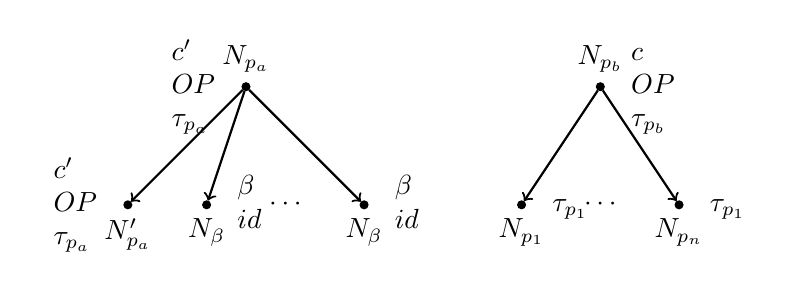
\begin{tikzpicture}[yscale=-1,
place/.style={circle,draw=black, fill=black, inner sep=0pt, 
              minimum size=1mm}]

  \node[place] (1st) at (1.5, 0) [label=above: $N_{p_a}$,
                                  label=left: 
     \begin{tabular}{l}
        $c'$\\
        $OP$\\
        $\tau_{p_a}$\\  
     \end{tabular}
] {};
  \node[place] (2nd) at (0, 1.5) [label=below: $N'_{p_a}$,
                                  label=left:
     \begin{tabular}{l}
        $c'$\\
        $OP$\\
        $\tau_{p_a}$\\  
     \end{tabular}
]{};
  \node[place] (3rd) at (1, 1.5) [label=below: $N_{\beta}$, 
    label=right: 
             \begin{tabular}{l}
            $\beta$\\
            $id$\\
             \end{tabular}
	] {}; 
  \node[place] (4th) at (3, 1.5) [label=below: $N_{\beta}$,
    label=right: 
             \begin{tabular}{l}
            $\beta$\\
            $id$\\
             \end{tabular}
             ] {}; 

  \node (dots) at (2,1.5) {$\cdots$};
	
  \draw[->, thick] (1st) -- (2nd);
  \draw[->, thick] (1st) -- (3rd);
  \draw[->, thick] (1st) -- (4th);

\begin{scope}[xshift=5cm]
  \node[place] (1st) at (1, 0) [label=above: $N_{p_b}$,
                                label=right: 
     \begin{tabular}{l}
        $c$\\
        $OP$\\
        $\tau_{p_b}$\\
     \end{tabular}
] {};
  \node[place] (2nd) at (0, 1.5) [label=below: $N_{p_1}$, 
    label=right: 
             \begin{tabular}{l}
            $\tau_{p_1}$\\
             \end{tabular}
             ] {};
  \node[place] (3rd) at (2, 1.5) [label=below: $N_{p_n}$, 
  label=right: 
             \begin{tabular}{l}
            $\tau_{p_1}$\\
             \end{tabular}
             ] {}; 

  \node (dots) at (1,1.5) {$\cdots$};
	
  \draw[->, thick] (1st) -- (2nd);
  \draw[->, thick] (1st) -- (3rd);
\end{scope}

);
\end{tikzpicture}
\end{center}
\caption{Comparison between atomic and complex predicates}
\label{fig:SimAC}
\end{figure}   % Picture

   \end{enumerate}
 
 \item \textit{complex predicate VS complex predicate}

   $p_a$ and $p_b$ are complex predicates with $\tau_{p_a}$ and $\tau_{p_b}$ as \textit{type}, respectively. If $p_a$ and $p_b$ are of the different \textit{types}, that is, $\tau_{p_a} \neq \tau_{p_b}$, then $Sim(p_a, p_b)=(-\infty,0)$ will be returned, otherwise, the expanding procedure will be carried on according to the fuzzy rules.
    $p_a$ is defined by rule
    \[p_a(\vec{t}) \stackrel{c^a,F_c^a}{\longleftarrow}F^a(p_1^a(\vec{t_1^a}),...,p_n^a(\vec{t_n^a}))\]
    with $OP_a=(F_c^a,F^a)$
    and $p_b$ is defined by rule
    \[p_b(\vec{t}) \stackrel{c^b,F_c^b}{\longleftarrow}F^b(p_1^b(\vec{t_1^b}),...,p_m^b(\vec{t_m^b}))\]
    with $OP_b=(F_c^b,F^b)$. There are two cases of $p_a$ and $p_b$ expansion.
   \begin{enumerate}
    \item $p_a$ and $p_b$ are defined by the different $OP$
     
     If $OP_a \neq OP_b$, which is, $F_c^a \neq F_c^b$ or $F^a \neq F^b$, then return $0$ as similarity degree, and $Sim(p_a, p_b)=(-\infty,0)$. 
   
    \item $p_a$ and $p_b$ are defined by the same $OP$
   
     If $OP_a=OP_b$, which is $F_c^a=F_c^b$ and $F^a=F^b$, then
     same two steps are taken here,
    \begin{itemize}
     \item Return middle result $Sim(p_a,p_b)=(l,u)$
     \item Continue the identity formalization, after which, $p_a$ and $p_b$ have corresponding trees with the same construction, where the roots are of the same type, the same $OP$, and have the same number of children. The comparing procedure of their children is recursively defined.
\end{itemize}
   \end{enumerate}

\begin{figure}[h!]
\begin{center}
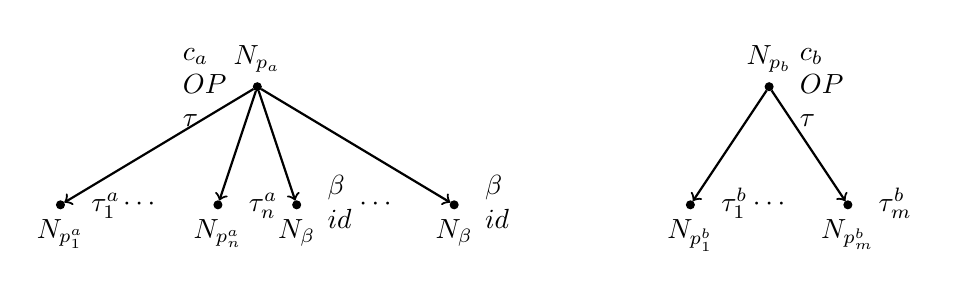
\begin{tikzpicture}[yscale=-1,
place/.style={circle,draw=black, fill=black, inner sep=0pt, 
              minimum size=1mm}]

  \node[place] (1st) at (2.5, 0) [label=above: $N_{p_a}$,
                                label=left: 
    \begin{tabular}{l}
      $c_a$\\
      $OP$\\
      $\tau$\\ 
    \end{tabular}
] {};
  \node[place] (2nd) at (0, 1.5) [label=below:  $N_{p_1^a}$,
  	label=right:
    		\begin{tabular}{l}
    			 $\tau_1^a$\\ 
   		 \end{tabular} ] {};
  \node[place] (3rd) at (2, 1.5) [label=below:   $N_{p_n^a}$,    
  	label=right:   
   		\begin{tabular}{l}
       			$\tau_n^a$\\ 
    		\end{tabular}] {}; 
  \node[place] (4th) at (3, 1.5) [label=below:  $N_{\beta}$,
  	label=right:
  	\begin{tabular}{l}
     		$\beta$\\
     		$id$\\ 
    	\end{tabular}] {}; 
  \node[place] (5th) at (5, 1.5) [label=below:  $N_{\beta}$,
  label=right:
  	\begin{tabular}{l}
     		$\beta$\\
     		$id$\\ 
    	\end{tabular}] {}; 
  
  \node (dots) at (1,1.5) {$\cdots$};
  \node (dots) at (4,1.5) {$\cdots$};
	
  \draw[->, thick] (1st) -- (2nd);
  \draw[->, thick] (1st) -- (3rd);
  \draw[->, thick] (1st) -- (4th);
  \draw[->, thick] (1st) -- (5th);


\begin{scope}[xshift=8cm]
  \node[place] (1st) at (1, 0) [label=above: $N_{p_b}$,
                                label=right: 
       \begin{tabular}{l}
         $c_b$\\
         $OP$\\
         $\tau$\\
       \end{tabular}
] {};
  \node[place] (2nd) at (0, 1.5) [label=below:  $N_{p_1^b}$,
  label=right:
  \begin{tabular}{l}
     $\tau_1^b$\\ 
    \end{tabular}]{};
  \node[place] (3rd) at (2, 1.5) [label=below:  $N_{p_m^b}$,
  label=right:
  \begin{tabular}{l}
     $\tau_m^b$\\ 
    \end{tabular}] {}; 

  \node (dots) at (1,1.5) {$\cdots$};
	
  \draw[->, thick] (1st) -- (2nd);
  \draw[->, thick] (1st) -- (3rd);
\end{scope}

);
\end{tikzpicture}
\end{center}
\caption{Comparison between two complex predicates} 
\label{fig:SimCC}
\end{figure}
%picture

\end{itemize}

For each expansion, the middle result which is the similarity value before next expansion and comparison, must be returned to filter some pairs of corresponding trees to reduce unnecessary expansion or comparison. The middle result of one level is formalized as follow.

Suppose that $p_a$ and $p_b$ are on level $l$ in their own trees, and are satisfied expanding requirements with $n$ children for each.
After combination of their children, $n$ optimal $Sim(p_i^a,p_j^b)$ are returned and composed as a \textit{middle set} $M_s$. The possible values in $M_s$ are $(-\infty,0)$, $(l-1,sim\_degree)$, $(l-1,u)$, where $sim\_degree \in [0,1]$. There is one subset of $M_s$, called \textit{decision middle set}, defined as,
\begin{equation}\label{eq:DecisionMiddleSet}
M_{ds}=\{(level,degree)| level \neq -\infty, degree \neq u\}
\end{equation}
The \textit{middle result} is $M_r = (l-1,M_v)$, where $M_v$ is defined as, 
\begin{equation}\label{eq:MiddleResult}
M_v=\frac{\sum_{i=1}^{m} v_i+1-\lvert c^a-c^b\rvert}{n+1}
\end{equation}
where $m$ is the cardinality of $M_{ds}$, $v_i$ is an element in $M_{ds}$. 

There are three points to be emphasized.
\begin{enumerate}
\item Similarity between identity and an arbitrary predicate

	The purpose of introducing identity $\alpha$ for an operation $OP=(\hat{F_c},\hat{F})$ is to build two predicate tree in the same structure, where two predicate trees have the identical $OP$ and the same number of children. The procedure of reconstructing predicate tree with equivalence preserves the original semantics. When comparing identity $\alpha$ and an arbitrary predicate $p$, the similarity between them is defined as $Sim(\alpha, p) = (l, v)$, where $l$ is the level the identity is on, and $v$ is an arbitrary value in $[0,1]$. The value $v$ will not affect the decision of choosing the optimal combination. The reason is shown in next point. 
	 
\item The property of Middle Result

	The \textit{middle result} is an element in $\mathbb{Z}/\mathbb{Z^+} \times [0,1]$, which is a partial order. The combination with precedent \textit{middle result} is chosen to be optimal combination, which is used to the next expansion. There are three questions are answered here. 
\begin{enumerate}	
\item Is $v$ in $Sim(\alpha,p)=(l,v)$ will affect the decision of choosing the optimal combination ? 
\item Why does precedent \textit{middle result} decide the optimal combination ?
\item What is the meaning of  $1- \lvert c^a - c^b  \rvert$ ?
\end{enumerate}
 	\begin{itemize}
	
	\item The affect of $Sim(\alpha, p)=(l,v)$
		
		 Suppose that obtaining similarity between $p_a$ and $p_b$ needs expansion. $p_a$, $p_b$ has $x$ and $y$ children respectively, and $x>y$. By building equivalent predicate tree for $p_b$, $x-y$ identities $\alpha$ are added as extra children of $p_b$. In any combinations of $x$ children in $p_a$ and $x$ children in $p_b$,  the number of $Sim(\alpha, p)$ is the same, which is $x-y$. According to formula \ref{eq:MiddleResult}, $M_v$ is monotonic increase on $v_i$. So the value of $v$ in $Sim(\alpha, p)=(l,v)$ will not affect on choosing an optimal combination.
		 
	\item The optimal combination
	
		In formula \ref{eq:DecisionMiddleSet}, $(-\infty,0)$ and $(l-1,u)$ are excluded from \textit{decision middle set} $M_{ds}$. The cardinality $m$ of $M_{ds}$ will affect the \textit{middle result} $M_r=(l-1,M_v)$, since $M_v$ is monotonic increase on $m$.  $(-\infty,0)$ means two predicates are not comparable and $(l-1,u)$ means similarity of two predicates are not defined in level $l-1$. Thus, the combination with more comparable pairs of predicates and more pairs of predicates with defined similarity has precedent \textit{middle result}.
		
	\item similarity between credit value
	
		Credit value $c^a$ and $c^b$ are the trust degrees of fuzzy rules within head $p_a$ and $p_b$, respectively. They are values in unit interval $[0,1]$. We define the distance between 
$c^a$ and $c^b$ by $1-norm$, which is $\lvert c^a-c^b \rvert$. The similarity between them is  $1- \lvert c^a - c^b  \rvert$. $c^a$ and $c^b$ are considered as a special pair of combinations, whose similarity is counted into the middle result of similarity between $p_a$ and $p_b$.  
	\end{itemize}
	
\item The termination of algorithm
	
	For any comparing pair $(p_i^a,p_j^b)$ from children of $p_a$ and $p_b$, if $Sim(p_i^a,p_j^b)=(l-1,u)$, it means that $p_i^a$ and $p_j^b$ have the same type but the similarity degree have not been defined directly in the RFuzzy program, and it could be reached by expanding them according to certain rules. The expanding procedure could be continued until both comparing predicates are atomic, which makes the algorithm terminate.
\end{enumerate} 


The algorithm terminates \textbf{iff} the comparing trees of predicates are \textit{completely built}.

\begin{defin} \textbf{Completely Built}.
The two comparing predicates are represented as trees, and expanded and valued in synchronization with each other until no comparing value $(level,u)$ is returned. Then the comparing trees are \textit {completely built}. The \textbf{similarity degree} is calculated from leaves to root by the definition of \textit{middle value}, and the \textbf{level} is the lowest level of the comparing trees.
\end{defin}

\begin{ex}

Here is a short RFuzzy program from the example \ref{ConstructPredicateTree},
\begin{center}
\begin{tabular}{l l}
$has\_tasty\_food:$  & $(Restaurant)$\\

$has\_healthy\_food:$ &  $(Restaurant)$\\

$has\_good\_service:$  & $(Restaurant)$\\

$tasty\_restaurant:$  & $(Restaurant)$\\

$good\_restaurant:$  & $(Restaurant)$\\
\end{tabular}
\end{center}
\begin{tabular}{l l l}
$tasty\_restaurant(X)$ & $\stackrel{1.0,.}{\longleftarrow} prod$ & $has\_tasty\_food(X)$\\

$good\_restaurant(X)$ & $\stackrel{0.8,.}{\longleftarrow} prod$ & $has\_healthy\_food(X), has\_good\_service(X)$ \\

\end{tabular}
\[Sim(has\_healthy\_food, has\_tasty\_food) = 0.6\]

\end{ex}
The set of \textit{Atomic predicates} is $AP= \{has\_tasty\_food, has\_healthy\_food, \linebreak[4]has\_good\_service\}$, and the set of \textit{complex predicates} is $CP= \{tasty\_restaurant,  \linebreak[4]good\_restaurant\}$. They have the same \textit{type} `Restaurant'. There are two tasks as examples for gaining the similarity, one is between  $tasty\_restaurant$ and $has\_tasty\_restaurant$, and the other is between $tasty\_restaurant$ and  \linebreak[4]$good\_restaurant$.

\begin{itemize}
 \item $Sim(tasty\_restaurant,has\_tasty\_food)$

Since $tasty\_restaurant \in CP$, and $has\_tasty\_food \in AP$, the procedure of obtaining similarity follows the case ``atomic predicate VS complex predicate''.
In an abbreviation, $tr$ is represented as $tasty\_restaurant$, $htf$ is for $has\_tasty\_food$, $R$ means `Restaurant'.
\newpage
\begin{figure}[h!]
\begin{center}
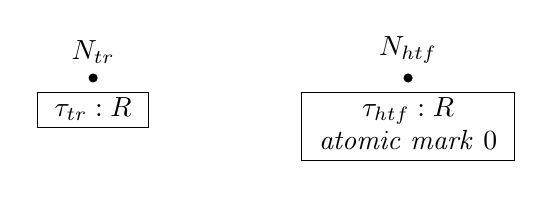
\begin{tikzpicture}[yscale=-1,
place/.style={circle,draw=black, fill=black, inner sep=0pt, 
              minimum size=1mm}]

 \node[place] (1st) at (1, 0) [label=above: $N_{tr}$,
                               label=below: 
            \begin{tabular}{|l|}
             \hline
             $\tau_{tr} : R$\\
             \hline
            \end{tabular}
] {};
	

\begin{scope}[xshift=4cm]
  \node[place] (1st) at (1, 0) [label=above: $N_{htf}$,
                               label=below: 
            \begin{tabular}{|c|}
              \hline
              $\tau_{htf} : R$\\
              \textit{atomic mark} 0\\
              \hline
            \end{tabular}] {};
\end{scope}


\end{tikzpicture}
\end{center}
\caption{Similarity between tr and htf}
\label{fig:SimTrHtf}
\end{figure}
For this pair of predicates, their \textit{types} are the same, that is, $\tau_{tr}=\tau_{htf}=R$. And, the similarity value between them is not directly defined in program. Then, two steps are taken afterwards,
\begin{enumerate}
 \item Return a middle result $Sim_{m}(tr,htf)=(0,u)$.
 \item Expand $tr$ and $htf$.     
 	\begin{figure}[h!]
\begin{center}
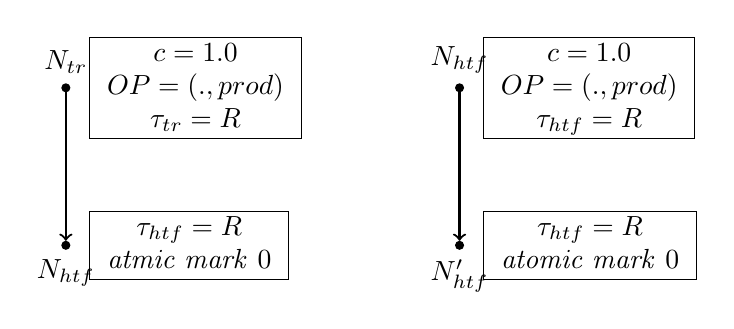
\begin{tikzpicture}[yscale=-1,
place/.style={circle,draw=black, fill=black, inner sep=0pt, 
              minimum size=1mm}]

\node[place] (1st) at (0, 0) [label=above: $N_{tr}$,
                              label=right: {
             \begin{tabular}{|c|}
               \hline
               $c=1.0$ \\
               $OP=(.,prod)$ \\
               $\tau_{tr}=R$ \\
               \hline
             \end{tabular} }] {};

\node[place] (2nd) at (0, 2) [label=below:  $N_{htf}$,
                                label=right: {
             \begin{tabular}{|c|}
               \hline
               $\tau_{htf}=R$\\
               \textit{atmic mark} $0$ \\
               \hline
             \end{tabular} }
] {};
        
	\draw[->, thick] (1st) -- (2nd);

\begin{scope}[xshift=5cm]
 \node[place] (1st) at (0, 0) [label=above: $N_{htf}$,
                              label=right: {
             \begin{tabular}{|c|}
               \hline
               $c=1.0$ \\
               $OP=(.,prod)$ \\
               $\tau_{htf}=R$ \\
               \hline
             \end{tabular} }] {};

\node[place] (2nd) at (0, 2) [label=below:  $N'_{htf}$,
                                label=right: {
             \begin{tabular}{|c|}
               \hline
               $\tau_{htf}=R$\\
               \textit{atomic mark} $0$\\
               \hline
             \end{tabular} }
] {};
        
	\draw[->, thick] (1st) -- (2nd);
\end{scope}

\end{tikzpicture}
\end{center}
\caption{Expansion of tr and htf}
\label{fig:ExpansionTrHtf}   
\end{figure} 
       According to the rule in program, which is 
       \begin{center}
         $tasty\_restaurant(X) \stackrel{1.0,.}{\longleftarrow} prod$ $has\_tasty\_food(X)$
       \end{center}
       $tr$ is expanded on the left of the figure \ref{fig:ExpansionTrHtf}, and according to $OP=(.,prod)$ from $tr$'s rule, $htf$ is expanded on the right side. As seen in the graph, only one combination of predicates in level $-1$ can be achieved, which is $(htf, htf)$. The similarity value of them is $(-1,1)$, since they are the same predicate, the similarity between them is $1$.  
\end{enumerate}
Thus, the similarity value is $1$ between $has\_tasty\_food$ and $tasty\_restaurant$ achieved in the level $-1$.

 \item $Sim(tasty\_restaurant,good\_restaurant)$
 
Since $tasty\_restaurant \in CP$, and so is $good\_restaurant$, the procedure of obtaining similarity follows the case ``complex predicate VS complex predicate''.
In an abbreviation, $tr$ is represented as $tasty\_restaurant$, $gr$ is for $good\_restaurant$, $R$ means `Restaurant'.
\begin{figure}[h!]
\begin{center}
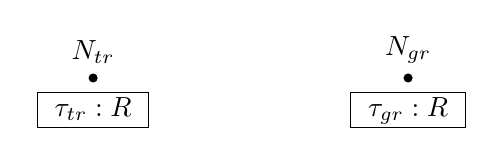
\begin{tikzpicture}[yscale=-1,
place/.style={circle,draw=black, fill=black, inner sep=0pt, 
              minimum size=1mm}]

 \node[place] (1st) at (1, 0) [label=above: $N_{tr}$,
                               label=below: 
            \begin{tabular}{|l|}
             \hline
             $\tau_{tr} : R$\\
             \hline
            \end{tabular}
] {};
	

\begin{scope}[xshift=4cm]
  \node[place] (1st) at (1, 0) [label=above: $N_{gr}$,
                               label=below: 
            \begin{tabular}{|c|}
              \hline
              $\tau_{gr} : R$\\
              \hline
            \end{tabular}] {};
\end{scope}


\end{tikzpicture}
\end{center}
\caption{Similarity between tr and gr} 
\label{fig:SimTrGr}  
\end{figure}
For this pair of predicates, their \textit{types} are the same, that is, $\tau_{tr}=\tau_{gr}=R$. And, the similarity value between them is not directly defined in RFuzzy program. Then, two steps are taken afterwards,
\begin{enumerate}
 \item Return a middle result $Sim_{m}(tr,gr)=(0,u)$.
 \item Expand $tr$ and $gr$. 
      \begin{figure}[h!]
\begin{center}
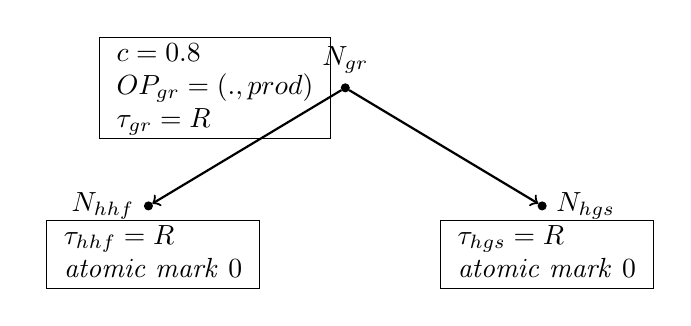
\begin{tikzpicture}[yscale=-1,
place/.style={circle,draw=black, fill=black, inner sep=0pt, 
              minimum size=1mm}]

  \node[place] (1st) at (2.5, 0) [label=above: $N_{gr}$,
                                  label=left: { 
             \begin{tabular}{|l|}
               \hline
               $c=0.8$\\
               $OP_{gr}=(.,prod)$\\
               $\tau_{gr}=R$\\
               \hline
             \end{tabular} }
] {};
	\node[place] (2nd) at (0, 1.5) [label=left: $N_{hhf}$,
                                        label=below: {
              \begin{tabular}{|l|}
                \hline
                 $\tau_{hhf}=R$ \\
                 \textit{atomic mark} $0$ \\
                \hline
              \end{tabular} }
             ] {};

        \node[place] (3rd) at (5, 1.5) [label=right: $N_{hgs}$, 
                                        label=below: {
              \begin{tabular}{|l|}
               \hline
               $\tau_{hgs}=R$ \\
               \textit{atomic mark} $0$ \\
               \hline
              \end{tabular} }
] {}; 

	\draw[->, thick] (1st) -- (2nd);
        \draw[->, thick] (1st) -- (3rd);
\end{tikzpicture}
\end{center}
\caption{Expansion of gr}
\label{fig:ExpansionGr}   
\end{figure}
       $gr$ is expanded acccording to the rule in program, which is 
      \begin{center}
       $good\_restaurant(X) \stackrel{0.8,.}{\longleftarrow} prod$ $has\_healthy\_food(X), has\_good\_service(X)$ 
      \end{center}
      According to the rule
      \begin{center}
         $tasty\_restaurant(X) \stackrel{1.0,.}{\longleftarrow} prod$ $has\_tasty\_food(X)$
      \end{center}
      and equivalence extension associated with $OP_{gr}$, the $tr$ is expanded into,
      \begin{figure}[h!]
\begin{center}
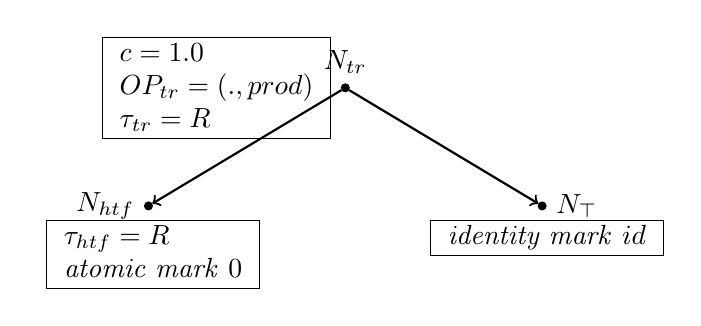
\begin{tikzpicture}[yscale=-1,
place/.style={circle,draw=black, fill=black, inner sep=0pt, 
              minimum size=1mm}]

  \node[place] (1st) at (2.5, 0) [label=above: $N_{tr}$,
                                  label=left: { 
             \begin{tabular}{|l|}
               \hline
               $c=1.0$\\
               $OP_{tr}=(.,prod)$\\
               $\tau_{tr}=R$\\
               \hline
             \end{tabular} }
] {};
	\node[place] (2nd) at (0, 1.5) [label=left: $N_{htf}$,
                                        label=below: {
              \begin{tabular}{|l|}
                \hline
                 $\tau_{htf}=R$ \\
                 \textit{atomic mark} $0$ \\
                \hline
              \end{tabular} }
             ] {};

        \node[place] (3rd) at (5, 1.5) [label=right: $N_{\top}$, 
                                        label=below: {
              \begin{tabular}{|l|}
               \hline
               \textit{identity mark} $id$ \\
               \hline
              \end{tabular} }
] {}; 

	\draw[->, thick] (1st) -- (2nd);
        \draw[->, thick] (1st) -- (3rd);
\end{tikzpicture}
\end{center}
\caption{Expansion of tr}
\label{fig:ExpansionTr}   
\end{figure}
       Two combinations of predicates in level $-1$ can be achieved, which are $M_{s_1}=\{(hhf,htf),(hgs,\top)\}$ and $M_{s_2}=\{(hgs,htf),(hhf,\top)\}$. In our program, only similarity between $has\_tasty\_food$ and $has\_healthy\_food$ is defined as \[Sim(has\_healthy\_food, has\_tasty\_food) = 0.6\]
       Suppose that for any predicate $p$, $Sim(\top,p)=0.5$, then the similarity achieved from $M_{s_1}$ is $M_{r_1}=(-1,0.6\dot{3})$ and from $M_{s_1}$ is $M_{r_2}=(-1,0.4\dot{3})$. The former combination $M_{s_1}$ will be chosen. In $M_{s_1}$, there is no $(l,u)$, which means no undefined similarity in this level $l$. Thus the comparing trees are \textit{completely built}, the algorithm terminates, and the similarity value is $0.63$ between $good\_restaurant$ and $tasty\_restaurant$ achieved in the level $-1$.       .  
\end{enumerate}

\end{itemize}


